\documentclass[10pt, AMS Euler]{article}
\textheight=9.25in \textwidth=7in \topmargin=-.75in
\oddsidemargin=-0.25in
\evensidemargin=-0.25in
\usepackage{url}  % The bib file uses this
\usepackage{graphicx} %to import pictures
\usepackage{amssymb, amsmath}
\usepackage{amsthm, concrete, multicol, color, wasysym}
\usepackage{tcolorbox}
\usepackage{tikz}
%\usepackage[normalem]{ulem} %for strikethrough (\sout{blah})
%\usepackage{tikz}
\usepackage{pgfplots}
\usepackage{array}

% adding hyperlinks
\usepackage{hyperref}

% for adding a ^ symbol as text
\usepackage{textcomp} % for \textasciicircum command

% for highlighting
\usepackage{soul}
\usepackage{xcolor}
\usepackage[utf8]{inputenc}
\usepackage{graphicx}

% for inserting code block (kinda)
\usepackage{listings}
\lstdefinestyle{python}{ 
    basicstyle=\ttfamily\footnotesize,
    breaklines=true,
    captionpos=b,
    commentstyle=\color{green},
    keywordstyle=\color{blue},
    numberstyle=\tiny\color{gray},
    stringstyle=\color{orange},
    language=Python,
}

\usetikzlibrary{shapes}
\usetikzlibrary{matrix}
\pgfplotsset{compat=1.14}
\pgfplotsset{rachel style/.append style={axis x line=middle, axis y line=
		middle, xlabel={$x$}, ylabel={$y$}}}
\pgfplotsset{time style/.append style={axis x line=middle, axis y line=
		middle, xlabel={$t$}, ylabel={$f(t)$}}}
\usetikzlibrary{arrows.meta}

% The following is needed for the figures
\usepackage{subfig}
\usetikzlibrary{positioning}
\usepackage{caption}
\usepgfplotslibrary{fillbetween}
%\numberwithin{figure}{section}
\captionsetup{width=.5\textwidth}
\pgfplotsset{
	cartesian style/.append style={axis x line=middle,
		axis y line= middle,
		xlabel={$x$}, ylabel={$y$}},
	midpoint segments/.code={\pgfmathsetmacro\integralsegments{#1}},
	midpoint sum/.style args={#1:#2}{
		ybar interval,
		domain=#1+((#2-#1)/\integralsegments)/2:#2+((#2-#1)/\integralsegments)/2,
		samples=\integralsegments+1,
		x filter/.code=\pgfmathparse{\pgfmathresult-((#2-#1)/\integralsegments)/2}
	}
}
% End of figures stuff

% A website with loads of examples:
% http://pgfplots.sourceforge.net/gallery.html

\usetikzlibrary{calc}


\setlength{\intextsep}{5mm} \setlength{\textfloatsep}{5mm}
\setlength{\floatsep}{5mm}


%%%%  SHORTCUT COMMANDS  %%%%
\newcommand{\ds}{\displaystyle}
\newcommand{\Z}{\mathbb{Z}}
\newcommand{\arc}{\rightarrow}
\newcommand{\R}{\mathbb{R}}
\newcommand{\N}{\mathbb{N}}
\newcommand{\Q}{\mathbb{Q}}
\newcommand{\C}{\mathbb{C}}
\newcommand{\stirling}[2]{\genfrac{\{}{\}}{0pt}{}{#1}{#2}}
\newcommand{\primes}{\mathscr{P}}

%%%%  footnote style %%%%

\renewcommand{\thefootnote}{\fnsymbol{footnote}}

\pgfplotsset{compat=newest}

\begin{document}
	
	
	\noindent{\bf \large Discrete Math 2: Experience Two}\\
    \noindent{\bf \large Brighton Ellis; Ann Marie Humble; Nate Stott} \\
	
	\noindent{\bf  Rules:} Complete the following problems by working in groups of at most three, and submit solutions (one document per group) typeset using \LaTeX by blah blah blah.\\


\subsection*{Sub-Experience 2.1.}
\textbf{Theorem 1: }
    Let $H$ be a vertex-transitive hypergraph and $e = \max\{|X| : X \in \mathcal{X}\}$. Then $k_f(H) = |S|/e$. \\\\

\textbf{Proof: }
    The constraint for each hyperedge $X$ in the IP (LP) formulation for $p(H)$ ($p_f(H)$) is $\sum_{s : s \in X} \nu(s) \leq 1$, where $s \in S$, and $\nu$ is a weight function defined on the vertices. If in the LP, we define $\nu(s) = 1/e$, this gives a feasible solution. Note that $1/e$ is the largest value we can use for a constant-valued feasible $\nu$. Therefore, $k_f(H) = p_f(H) \geq |S|/e$. 
    
    Now let $\Gamma$ denote the automorphism group of $H$, and suppose $\nu : S \rightarrow [0, 1]$ yields an optimal fractional packing of $H$. Let $\pi \in \Gamma$, and note that $\nu \circ \pi : S \rightarrow [0, 1]$ also yields an optimal fractional packing of $H$. Define $\nu^*(s) = \frac{1}{|\Gamma|} \sum_{\pi \in \Gamma} \nu(\pi(s))$ and note that this is simply a convex combination of functions that yield optimal fractional packings and so it too yields an optimal fractional packing. But since $H$ is vertex-transitive, $\nu^*$ assigns the same weight to each vertex $s$. Since, as noted above, $1/e$ is the largest value a constant-valued feasible function can assign, $p_f(H) = k_f(H) = |S|/e$. \\

\textbf{Corollary 2: }
The fractional biclique cover number of $K_n$ is $\binom{n}{2}/ab$, where $ab$ is the maximum number of edges in any biclique of $K_n$. \\

\textbf{proof}
    Let $H$ be the hypergraph whose vertices are edges of $K_n$ and whose hyperedges are the bicliques of $K_n$. The hypergraph $H$ is vertex-transitive because $K_n$ is edge-transitive. Apply the proposition, noting that the hyperedge vertex covering number of $H$ is the biclique cover number of $K_n$ in this case. \\



\textbf{Part 0}

Corollary 2 (you gave us this before you changed the draft): \\
\begin{align*}
    w(B) = 1 \text{number of bicliques with an edge} \\ 
    v(e) = 1 \text{number of edges in largest biclique)} \\
    \text{max} \sum_{e \in E} v(e) \text{ = (number of edges) / (number of edges in largest biclique) } = \binom{n}{2} \text{/ (number of edges in largest biclique)} \\
\end{align*}

\textbf{Part 1}

$bc^*(K_n) = \frac{\binom{n}{2}}{ab}$ where $ab$ is the number of edges in the largest biclique \\

So what is the size of the largest biclique? \\

$$ K_{\lceil \frac{n}{2} \rceil,  \lfloor \frac{n}{2} \rfloor } $$

\textbf{Part 2}

$$ a = \lceil \frac{n}{2} \rceil $$
$$ b = \lfloor \frac{n}{2} \rfloor $$

$$ ab = \lceil \frac{n}{2} \rceil * \lfloor \frac{n}{2} \rfloor $$

Well we gotta break up into some cases \\

$ = \frac{n^2}{4}$ n is even \\

$ = \frac{n^2-1}{4}$ n is odd \\

\textbf{Part 3}

Even Case: \\

$$ bc^*(K_n) = \frac{\binom{n}{2}}{\frac{n^2}{4}} $$
$$ = \frac{4\binom{n}{2}}{n^2} $$
$$ = \frac{2(n^2-n)}{n^2} $$
$$ = \frac{2(n-1)}{n} $$

So for the even case we got \\

$$ bc^*(K_n) = 2\frac{n-1}{n} $$

Odd Case: \\

$$ bc^*(K_n) = \frac{\binom{n}{2}}{\frac{n^2-1}{4}} $$
$$ = \frac{4\binom{n}{2}}{n^2-1} $$
$$ = \frac{2n(n-1)}{(n+1)(n-1)} $$
$$ = \frac{2n}{n+1} $$

So for the odd case we got \\

$$ bc^*(K_n) = \frac{2n}{n+1} $$

\textbf{Solution}

n Even \\
$$ bc^*(K_n) = 2\frac{n-1}{n} $$

n Odd \\
$$ bc^*(K_n) = \frac{2n}{n+1} $$

\begin{align*}
    \includegraphics[width=.6\textwidth]{imgs/bipartite-stuffs.png}
\end{align*}

------------------------------------

\subsection*{Sub-Experience 2.2.}
A hypergraph $H = (S, \mathcal{X})$ is set system with vertex set $S$ and hyperedge set $\mathcal{X}$, where $\mathcal{X}$ consists of subsets of $S$. A hyperedge vertex cover of hypergraph $H$ is a set of hyperedges $X_1, X_2, \ldots, X_m$ that contain $S$. Define $k(H)$ to be the smallest $m$ for which there exists a set of $m$ hyperedges that contain $S$. Computing $k(H)$ can be formulated as an IP and hence can be relaxed to an LP; the relaxation is denoted $k_f(H)$ and is called the fractional hyperedge vertex cover of $H$. The IP $k(H)$ has a dual: the packing number of $H$, denoted $p(H)$. That is, $p(H)$ is the maximum number of vertices of $H$, no two of which belong to the same hyperedge. The packing number, of course, can be relaxed to an LP, the fractional packing number of $H$, denoted $p_f(H)$. By weak duality we have $p_f(H) \leq k_f(H)$, and by strong duality we have $p_f(H) = k_f(H)$.

The Fano Plane is one of the niftiest$^*$ objects in Combinatorics. It can be defined to be the hypergraph $H$ with vertex set $S = \{1, 2, 3, 4, 5, 6, 7\}$, and hyperedges

\[
\mathcal{X} = \bigl\{\{1, 2, 3\}, \{1, 4, 5\}, \{2, 4, 6\}, \{3, 4, 7\}, \{2, 5, 7\}, \{1, 6, 7\}, \{3, 5, 6\}\bigr\}.
\]

It is also the projective plane of order 2, the finite difference set called "(7, 3, 1)", and it is equivalent to the skew Hadamard matrix of order 8. \ldots\ Anyway \ldots\ the Fano Plane is depicted below.

\begin{align*}
    \includegraphics[width=0.3\textwidth]{imgs/Fano-Plane.png}
\end{align*}

Please determine the covering number, packing number, fractional covering number, and fractional packing number of the Fano Plane; that is, determine $k(H)$, $p(H)$, $k_f(H)$, and $p_f(H)$.

\footnotetext{$^*$Intentionally vague.}

% Nate will write this up I got it I just wrote notes to remind myself

Pick a node and cross out the nodes on the same hyperedge. What is the max number of vertices you can pick?

In order to find the packing number, combinatorially we can pick a vertex (any vertex) and then cross out any nodes that are touched by the hyperedges that also connect to that chosen node.  A visual representation is provided below.
\begin{align*}
    \includegraphics[width=.3\textwidth]{imgs/fanoPack.png}
\end{align*}
In this visual representation, we can see that every vertex can be reached from the hyperedges of any chosen vertex. Therefore, the packing number maxes out at $1$.
$$ p(H) = 1 $$

How many edges can you get by doing a similar idea as above 
% begin legit explanation:
let's think about it combinatorially. Each hyperedge consists of 3 vertices. With the Fano Plane representing $7$ vertices, then at a minimum we would need 3 different hyperedges in order to cover all 7 vertices. Ex. 1 hyperedge = 3 vertices, 2 hyperedges = 6 vertices, 3 hyperedges= up to 9 vertices. Now lets double check that that works out on our actual graph
\begin{align*}
    \includegraphics[width=.3\textwidth]{imgs/fanoKoverProof.png}
\end{align*}
This is the minimum number of hyperedges that we can use to cover all of the vertices. Other possible hyperedge combinations would only essentially be rotations on the colored hyperedges above. so, the cover number for this is $3$ 
$$ k(H) = 3 $$



Matrix is the same if you T. p and k are primal and dual. Set each edge to 1/3


\begin{center}
    \begin{table}[htbp]
    \centering
    \begin{tabular}{c|ccccccc}
    & E1 & E2 & E3 & E4 & E5 & E6 & E7 \\ \hline
    1 & 1 & 1 & 1 & 0 & 0 & 0 & 0 \\
    2 & 1 & 0 & 0 & 1 & 1 & 0 & 0 \\
    3 & 1 & 0 & 0 & 0 & 0 & 1 & 1 \\
    4 & 0 & 1 & 0 & 1 & 0 & 1 & 0 \\
    5 & 0 & 1 & 0 & 0 & 1 & 0 & 1 \\
    6 & 0 & 0 & 1 & 1 & 0 & 0 & 1 \\
    7 & 0 & 0 & 1 & 0 & 1 & 1 & 0 \\
    \end{tabular}
    \caption{adjacency matrix}
    \label{tab:my-table}
    \end{table}
\end{center}

We notice that the adjacency matrix is diagonal symmetric. Or rather, that the transpose of the matrix will be identical to before the transposition.  This works out for our convenience because the solving of the equation for the dual will be identical for that of the primal, meaning that we can get the same answer for the fractional primal as well as the fractional dual. 

thus $1^Tv =\frac{7}{3}$ is solution for the LP     \\
$$ p_f(H) = \frac{7}{3} $$



\begin{center}
    $
    \begin{bmatrix}
    1 & 1 & 1 & 1 & 0 & 0 & 0 \\
    1 & 0 & 0 & 1 & 1 & 0 & 0 \\
    1 & 0 & 0 & 0 & 0 & 1 & 1 \\
    0 & 1 & 0 & 1 & 0 & 1 & 0 \\
    0 & 1 & 0 & 0 & 1 & 0 & 1 \\
    0 & 0 & 1 & 1 & 0 & 0 & 1 \\
    0 & 0 & 1 & 0 & 1 & 1 & 0 \\
    \end{bmatrix}
    \cdot
    \begin{bmatrix}
    \frac{1}{3} \\
    \frac{1}{3} \\
    \frac{1}{3} \\
    \frac{1}{3} \\
    \frac{1}{3} \\
    \frac{1}{3} \\
    \frac{1}{3} \\
    \end{bmatrix}
    =
    \begin{bmatrix}
    1 \\
    1 \\
    1 \\
    1 \\
    1 \\
    1 \\
    1 \\
    \end{bmatrix}    
    $
\end{center}

% ---------------------------------------------
    %  This is where the equations for the next 2 parts of the problem will go. 
% ---------------------------------------------
in the same way, we can see that $ M^Tv \leq 1 $

\begin{center}
    $
    \begin{bmatrix}
    1 & 1 & 1 & 1 & 0 & 0 & 0 \\
    1 & 0 & 0 & 1 & 1 & 0 & 0 \\
    1 & 0 & 0 & 0 & 0 & 1 & 1 \\
    0 & 1 & 0 & 1 & 0 & 1 & 0 \\
    0 & 1 & 0 & 0 & 1 & 0 & 1 \\
    0 & 0 & 1 & 1 & 0 & 0 & 1 \\
    0 & 0 & 1 & 0 & 1 & 1 & 0 \\
    \end{bmatrix}
    \cdot
    \begin{bmatrix}
    \frac{1}{3} \\
    \frac{1}{3} \\
    \frac{1}{3} \\
    \frac{1}{3} \\
    \frac{1}{3} \\
    \frac{1}{3} \\
    \frac{1}{3} \\
    \end{bmatrix}
    =
    \begin{bmatrix}
    1 \\
    1 \\
    1 \\
    1 \\
    1 \\
    1 \\
    1 \\
    \end{bmatrix}    
    $
\end{center}

$$ k_f(H) = \frac{7}{3} $$

-------------------------------

\subsection*{Sub-Experience 2.3.}
	
	\noindent First, I'll entreat you to some definitions.  
	The {\bf adjacency matrix} of directed graph $D = (\{v_1, \dots, v_n\},A)$ is the matrix $[D]$ in which entry $(i,j)$ is $1$ if $v_i \to v_j$ in $D$ and is zero other wise\footnote{The notation ``$a \to b$'' is the shorthand I use to indicate there is an arc \emph{from} $a$ \emph{to} $b$.  Equivalently, saying ``$a \to b$ in $D = (V,A)$'' means ``$(a,b) \in A$''.}. 
	The {\bf Boolean rank} of $\{0,1\}$-matrix $M$, denoted $r_{B}(M)$, is the minimum number of rank-1 matrices (of the same size as $M$) whose sum is $M$ using Boolean arithmetic.  
	Equivalently, for whatever this is worth, the {\bf Boolean rank} of the $m \times n$ $\{0,1\}$-matrix $M$ is the minimum $k$ for which there is an $m \times k$ matrix  $A$ and a $k \times n$ matrix $B$ for which $M  = AB$ using Boolean arithmetic.  
	By the way, ``Boolean arithmetic'' means the numbers you work with are $0$ and $1$ and all operations are the same as with integers or rationals except $1+1=1$.  
	There are no negative numbers in Boolean arithmetic, so you cannot solve an equation such as $x +1 = 1$. 
	The {\bf isolation number} of a matrix $M$, denoted $\iota(M)$ is the maximum number of nonzero entries such that no two belong to the same row, no two belong to the same column, and no two belong to a submatrix of the form ${\footnotesize \left[\begin{array}{cc} 1 & 1 \\ 1 & 1\end{array} \right]}$. 
	Note that the submatrix may be  the intersection of any pair of columns and any pair of rows. 
	As examples, consider the following: $\iota(A) = 1$, $\iota(B) = 1$, $\iota(C) = 5$, and $\iota(D) =3$.
	$$A = \left[\begin{array}{cccccc} 1 & 0 & 0 & 0 & 0 & 1 \\ 
		0 & 0 & 0 & 0 & 0 & 0 \\
		0 & 0 & 0 & 0 & 0 & 0 \\
		1 & 0 & 0 & 0 & 0 & 1 \end{array} \right] \hspace{0.15in} 
	B = \left[\begin{array}{cccccc} 1 & 1 & 1 & 1 & 1 & 1 \\ 
		1 & 1 & 1 & 1 & 1 & 1 \\
		1 & 1 & 1 & 1 & 1 & 1 \\
		1 & 1 & 1 & 1 & 1 & 1 \\
		1 & 1 & 1 & 1 & 1 & 1 \end{array} \right] \hspace{0.15in} 
	C = \left[\begin{array}{ccccc} 1 & 0 & 0 & 0 & 0  \\ 
		1 & 1 & 0 & 0 & 0 \\
		1 & 1 & 1 & 0 & 0  \\
		1 & 1 & 1 & 1 & 0 \\
		1 & 1 & 1 & 1 & 1 \end{array} \right]\hspace{0.15in} 
	D = \left[\begin{array}{ccccc} 0 & 1 & 1 & 1 & 1  \\ 
		1 & 0 & 1 & 1 & 1 \\
		1 & 1 & 0 & 1 & 1  \\
		1 & 1 & 1 & 0 & 1 \\
		1 & 1 & 1 & 1 & 0 \end{array} \right]$$ 
	
	
	\noindent Please prove the following lemma: \\
	
	\noindent{\bf Lemma 2.3.1.} \emph{For any $\{0,1\}$-matrix $M$, $\iota(M) \leq r_B(M)$.}\\

    Start Proof
    
    Rank number: the number of linearly independent columns
    Isolation number: the maximum number of 1s in the matrix that don't share a row or column with each other or don't create a 2 by 2 matrix of ones.
    
    If you start with the identity matrix, then the rank and isolation are equal. If you add ones to a column such that, that column is now the same as another column, then those columns are no longer linearly independent. If they are not linearly independent, then you will have a one's square. And that will cause the isolation number to go down. Therefore, the only way to decrease the rank is to decrease the isolation number. 

    However, if you place once such that it creates a one's square, but columns remain linearly independent, then the isolation number has decreased without decreasing the rank.

    Therefore, the isolation number will always be less than or equal to the rank.

    We are very confident that this is true.

    End Proof
	
	Consider the directed graph (which is a \emph{tournament}) depicted below; call it $T$, and denote its adjacency matrix by $[T]$. 
	
	\begin{center}
		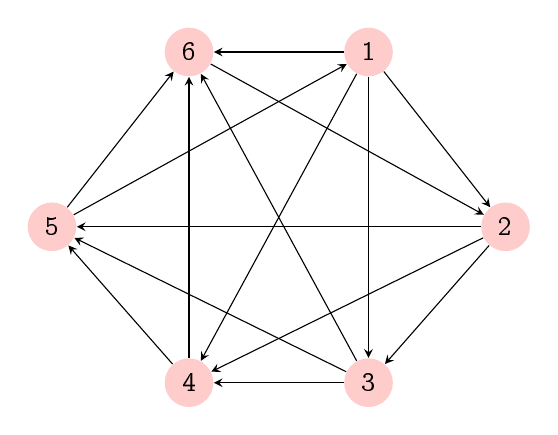
\begin{tikzpicture}[scale=0.6, every node/.style={circle, fill=red!20}]
			
			\node (n1) at (1.9, 3.5) {1};
			\node (n2) at (4.8, -0.2) {2};
			\node (n3) at (1.9, -3.5)  {3};
			\node (n4) at (-1.9, -3.5)  {4};
			\node (n5) at (-4.8, -0.2)  {5};
			\node (n6) at (-1.9, 3.5) {6};
			
			%  for n1
			\draw[-stealth] (n1) -- (n2);
			\draw[-stealth] (n1) -- (n3);
			\draw[-stealth] (n1) -- (n4);
			\draw[-stealth] (n1) -- (n6);
			%  for n2
			\draw[-stealth] (n2) -- (n3);
			\draw[-stealth] (n2) -- (n4);
			\draw[-stealth] (n2) -- (n5);
			
			%  for n3
			\draw[-stealth] (n3) -- (n4);
			\draw[-stealth] (n3) -- (n5);
			\draw[-stealth] (n3) -- (n6);
			%  n4
			\draw[-stealth] (n4) -- (n5);
			\draw[-stealth] (n4) -- (n6);
			%  for n5
			\draw[-stealth] (n5) -- (n1);
			\draw[-stealth] (n5) -- (n6);
			% for n6
			\draw[-stealth] (n6) -- (n2);
		\end{tikzpicture}
	\end{center}
	
	\noindent Please determine the Boolean rank and isolation number of $[T]$.\\

    After much deliberation, we came to the conclusion of the numbers below. \\

    Also though, here's our reasoning:\\

    The biclique cover number of a graph is going to be the same as that graph's boolean rank. If you write out the adjacency matrix of this graph, you will see that the graph can be broken down into five linearly independent vectors. This means that the biclique cover number of this graph is five (one for each linearly independent vector) and thus the boolean rank of this graph is five. \\
    
    Another way to think about this is breaking the matrix up into a sum of outer products. \\

    Here is an example of what we did to solve the problem. \\

    \includegraphics[width=.5\textwidth]{imgs/math.jpeg}

    Also, here's what we actually did:\\
    Here's the adjacency matrix we started with:\\
    \begin{bmatrix}
        0 & 1 & 1 & 1 & 0 & 1 \\
        0 & 0 & 1 & 1 & 1 & 0 \\
        0 & 0 & 0 & 1 & 1 & 1 \\
        0 & 0 & 0 & 0 & 1 & 1 \\
        1 & 0 & 0 & 0 & 0 & 1 \\
        0 & 1 & 0 & 0 & 0 & 0 \\
    \end{bmatrix}
    \\

    Here's the boolean rank solved for:\\

    \includegraphics[width=1\textwidth]{imgs/math1.jpg}

    To find the isolation number of the graph, look at the matrix again and just see how many 1's you can get that are isolated from each other. The 1's won't be isolated if they could form a 2 by 2 sub-matrix with each other.\\

    $$ i(T) = 5 $$

    $$ r_b(T) = 6 $$
	
	\noindent Now consider the tournament depicted below, call it $DR_7$ because of ... reasons. 
	
	\begin{center}
		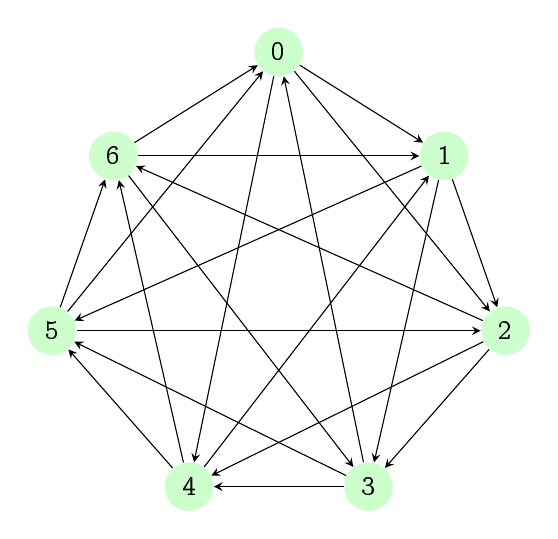
\begin{tikzpicture}[scale=0.6, every node/.style={circle, fill=green!20}]
			\node (n0) at (0, 5.7) {0};
			\node (n1) at (3.5, 3.5) {1};
			\node (n2) at (4.8, -0.2) {2};
			\node (n3) at (1.9, -3.5)  {3};
			\node (n4) at (-1.9, -3.5)  {4};
			\node (n5) at (-4.8, -0.2)  {5};
			\node (n6) at (-3.5, 3.5) {6};
			% all 6 for n0
			\draw[-stealth] (n0) -- (n1);
			\draw[-stealth] (n0) -- (n2);
			\draw[stealth-] (n0) -- (n3);
			\draw[-stealth] (n0) -- (n4);
			\draw[stealth-] (n0) -- (n5);
			\draw[stealth-] (n0) -- (n6);
			% 5 other for n1
			\draw[-stealth] (n1) -- (n2);
			\draw[-stealth] (n1) -- (n3);
			\draw[stealth-] (n1) -- (n4);
			\draw[-stealth] (n1) -- (n5);
			\draw[stealth-] (n1) -- (n6);
			% 4 other for n2
			\draw[-stealth] (n2) -- (n3);
			\draw[-stealth] (n2) -- (n4);
			\draw[stealth-] (n2) -- (n5);
			\draw[-stealth] (n2) -- (n6);
			% 3 other for n3
			\draw[-stealth] (n3) -- (n4);
			\draw[-stealth] (n3) -- (n5);
			\draw[stealth-] (n3) -- (n6);
			% 2 other for n4
			\draw[-stealth] (n4) -- (n5);
			\draw[-stealth] (n4) -- (n6);
			% 1 last for n5
			\draw[-stealth] (n5) -- (n6);
		\end{tikzpicture}
	\end{center}
	
	\noindent Please determine the Boolean rank and isolation number of $[DR_7]$.\\

    After much deliberation, we came to the conclusion of the numbers below.\\

    Here is the adjacency matrix we used:\\

    \begin{bmatrix}
        0 & 1 & 1 & 0 & 1 & 0 & 0 \\
        0 & 0 & 1 & 1 & 0 & 1 & 0 \\
        1 & 0 & 0 & 0 & 1 & 1 & 0 \\
        1 & 0 & 0 & 0 & 1 & 1 & 0 \\
        0 & 1 & 0 & 0 & 0 & 1 & 1 \\
        1 & 0 & 1 & 0 & 0 & 0 & 1 \\
        1 & 1 & 0 & 1 & 0 & 0 & 0 \\
    \end{bmatrix}
    \\

    We used the same methodology as with the graph above to solve this one.
    
     $$ i(DR_7) = 7 $$
     
     $$ b_r(DR_7) = 7 $$
	
	\begin{center}
		{\Large \textsc{The end}}
	\end{center}
	
	\noindent Postscript: The references below are provided in case you want to read the original stuff on the stuff in the first prompt on (non-fractional) biclique covers of the complete graph. 
	Also, there's one of my papers on Boolean ranks of tournament matrices \cite{BroRoy} \smiley. 
	
	\begin{thebibliography}{99}
		
		\bibitem{BezFroRosKov}
		Bezrukov, S.,  D. Fron\v{c}ek, S. J. Rosenberg, P. Kov\'{a}\v{r}, On biclique coverings, \emph{Discrete Math.}, {\bf 308} (2008) 319 -- 323.
		
		\bibitem{BroRoy}
		Brown, D. E., S. Roy, J. R. Lundgrem, D.J. Siewert, Boolean rank of upset tournament matrices, \emph{Linear ALgebra and its Applications}, {\bf 436:9} (2012) 3239 -- 3246.
		
		\bibitem{deCGrePul}
		de Caen, D.,D. Gregory, N. Pullman, The Boolean rank of zero one matrices, \emph{Proc. Third Caribbean Conf. on Combinatorics and Computing, Barbados},
		(1981), 169 -- 173.
		
		\bibitem{FronJerKlaKov}
		Fron\v{c}ek, D., J. Jerebic, S. Klav\v{z}ar, P. Kov\'{a}\v{r}, Strong isoperimetric dimension, biclique coverings, and Sperner's Theorem,
		\emph{Combin. Prob. and Comput.}, {\bf 16} (2007) 271 -- 275.
		
		\bibitem{GraPol}
		Graham, R. L., H. O. Pollak. On embedding graphs in squashed cubes. In: \emph{Graph Theory and Appl., Springer Lecture Notes in Math.}
		{\bf 303} (1972), 99 -- 110.
		
		%\bibitem{SchUllFGT}
		%Scheinerman, E. R., D. H. Ullman, \emph{Fractional Graph Theory: A Rational Approach to the Theory of Graphs}, Wiley \& Sons, 2004.
		
		\bibitem{ZhaCui}
		Zhang, G.-Q., L. Cui, A set coverage problem, \emph{Inform. Process. Lett.}, {\bf 110:4} (2010) 158 -- 159.
		
	\end{thebibliography}



\end{document}